\documentclass[12pt]{article}
\usepackage{amsmath}
\usepackage{latexsym}
\usepackage{amsfonts}
\usepackage{amssymb}
\usepackage{graphicx}
\usepackage{txfonts}
\usepackage{wasysym}
\usepackage{adjustbox}
\usepackage{ragged2e}
\usepackage{tabularx}
\usepackage{hhline}
\usepackage{float}
\usepackage{multirow}
\usepackage{makecell}
\usepackage{fancyhdr}
\usepackage[utf8]{inputenc}
\usepackage[T1]{fontenc}
\usepackage{listings}

\usepackage{syntax}

\usepackage[a4paper,bindingoffset=0.2in,headsep=0.5cm,left=1in,right=1in,bottom=3cm,top=2cm,headheight=2cm]{geometry}
\usepackage{hyperref}
\usepackage{listings}
\usepackage[most]{tcolorbox}

\lstset{language=C,basicstyle=\scriptsize\ttfamily,keywordstyle=\bfseries, commentstyle=\textit,stringstyle=\ttfamily, showspaces=false,showstringspaces=false, frame=single,
  breaklines=true,
  postbreak=\mbox{\textcolor{red}{$\hookrightarrow$}\space},
}

\everymath{\displaystyle}
\pagestyle{fancy}
\fancyhf{}
\rfoot{Page \thepage}
\begin{document}
\sloppy 

\begin{center}


\includegraphics[width=0.2\textwidth]{fig/tp}
\vspace{10 pt}\\
\Huge TTool \\
\vspace{10 pt}
\Large \url{ttool.telecom-paris.fr}
\vspace{20 pt}\\
\underline{\Large Use of TTool explained through the creation of a coffee machine.}
\vspace{30 pt}
\end{center}

\begin{table}[H]
\large
\centering
\begin{adjustbox}{width=\textwidth}
\begin{tabular}{ |p{1.6cm}|p{6.0cm}|p{4.2cm}|p{4.2cm}| }
\hhline{----}
 & \textbf{Document Manager} & \textbf{Contributors}  & \textbf{Checked by}  \\ 
\hhline{----}
\textbf{Name}   & Ludovic APVRILLE & \multirow{2}{4.2cm}{Christophe Manseau, Philippe Paquette,
Ludovic APVRILLE} &
\multirow{2}{*}{Ludovic APVRILLE} \\
\hhline{--~~}
\textbf{Contact} & ludovic.apvrille@telecom-paris.fr &  &  \\ 
\hhline{--~~}
\textbf{Date} & \today &  &  \\ 
\hline
\end{tabular}
\end{adjustbox}
\end{table}

\newpage
\tableofcontents

% \newpage
% \listoffigures

\newpage
\section{Preface}

\subsection{Table of Versions}

\begin{table}[H]
\large
\centering
\begin{adjustbox}{width=\textwidth}
\begin{tabular}{ |p{1.5cm}|p{2.5cm}|p{9.0cm}|p{3.0cm}| }
\hhline{----}
\textbf{Version} & \textbf{Date} & \textbf{Description  $  \&  $  Rationale of
Modifications} & \textbf{Sections Modified} \\
\hhline{----}
1.0 & July 7, 2018 & First draft &  \\ 
\hline
1.1 & Oct 29, 2019 & Adding safety pragmas &  \\ 
\hline
\end{tabular}
\end{adjustbox}
\end{table}

\subsection{Table of References and Applicable Documents}

\begin{table}[H]
\large
\centering
\begin{adjustbox}{width=\textwidth}
\begin{tabular}{ |p{2.66in}|p{2.66in}|p{0.95in}|p{0.43in}| }
\hhline{----}
\textbf{Reference} & \textbf{Title  $  \&  $  Edition} & \textbf{Author or
Editor} & \textbf{Year}
\\
\hhline{----}
 &  &  &  \\ 
\hline
\end{tabular}
\end{adjustbox}
\end{table}

\subsection{Acronyms and glossary}

\begin{table}[H]
\large
\centering
\begin{adjustbox}{width=\textwidth}
\begin{tabular}{ |p{1.24in}|p{5.45in}| }
\hhline{--}
\textbf{Term} & \textbf{Description} \\ 
\hhline{--}
 &  \\ 
\hline
\end{tabular}
\end{adjustbox}
\end{table}

\newpage
\section{Introduction}

TTool is an open-source toolkit dedicated to the design of embedded systems based on UML and SysML diagrams. The source files of TTool can be downloaded from the website: http://ttool.telecom-paris.fr/download.html
after having accepted the license agreement. To install the tool, simply unpack the archive in your home directory and follow the installation process of your operating system.

\section{Getting Started}
\subsection{Opening from terminal}

After downloading it from the Internet, the most effective way to open TTool is to open it from your computer terminal. Open the folder in which the application is located and then open using the command:
\begin{lstlisting}{bash}

 start ttool_windows
 

\end{lstlisting}

or 
\begin{lstlisting}{bash}

open ttool_macosx
 

\end{lstlisting}

or \begin{lstlisting}{bash}

Run ttool_linux

\end{lstlisting}


\subsection{Start new project}
To create a new project, click on the “new” button as shown in Figure \ref{fig:createfile} below or select file and then new on the main tab. As shown in Figure \ref{fig:createmethod}, the main TTool window contains three different areas, the Project navigation window, the Design window and the Map view window; allowing the user to navigate through the files of the project and rapidly search for elements of a design, observe and create the SysML diagrams of the design, and have a bird’s eye view of the current diagram respectively.

\begin{figure*}[htbp]
\centering
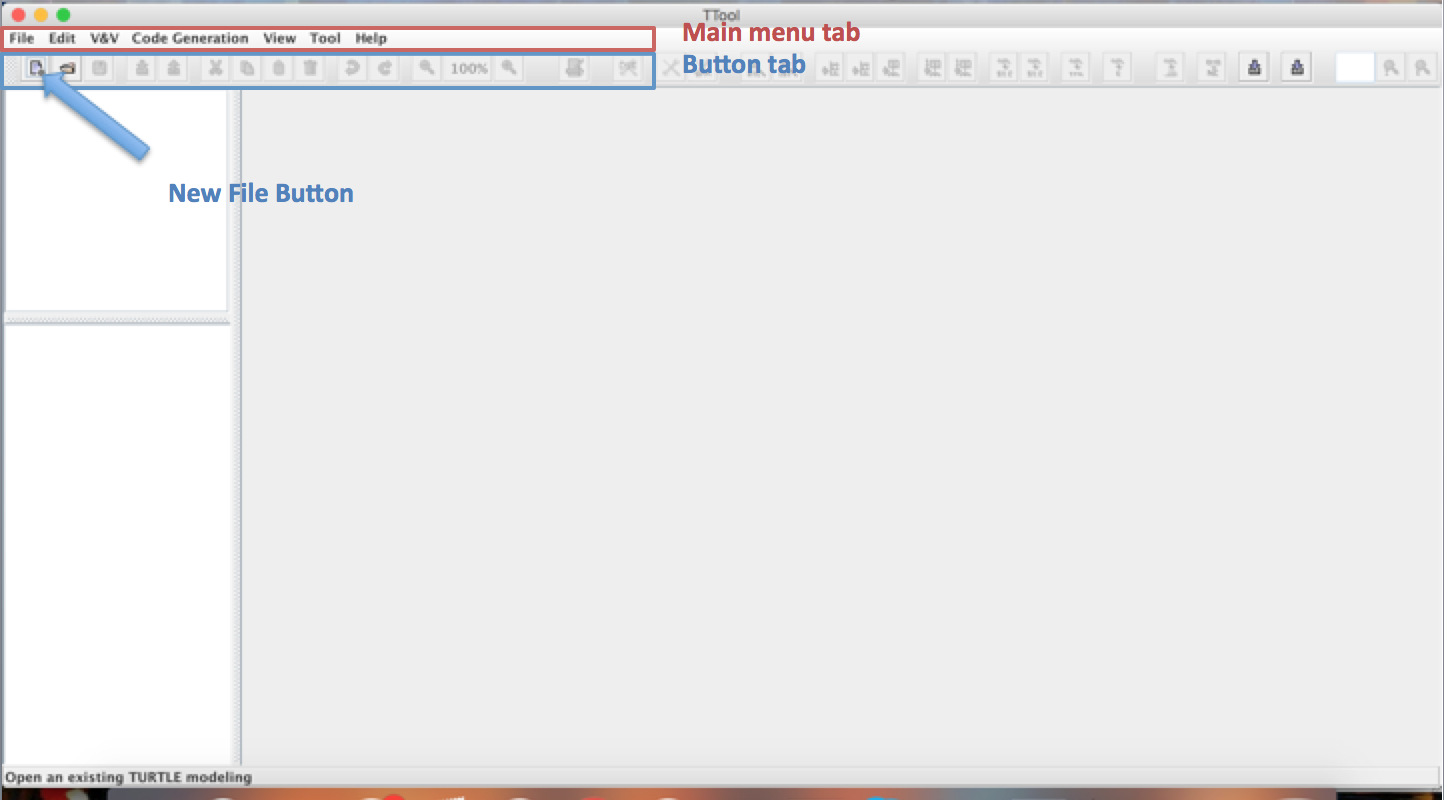
\includegraphics[width=0.99\textwidth]{fig/createfile.png}
\caption{Create a file} \label{fig:createfile}
\end{figure*}

\begin{figure*}[htbp]
\centering
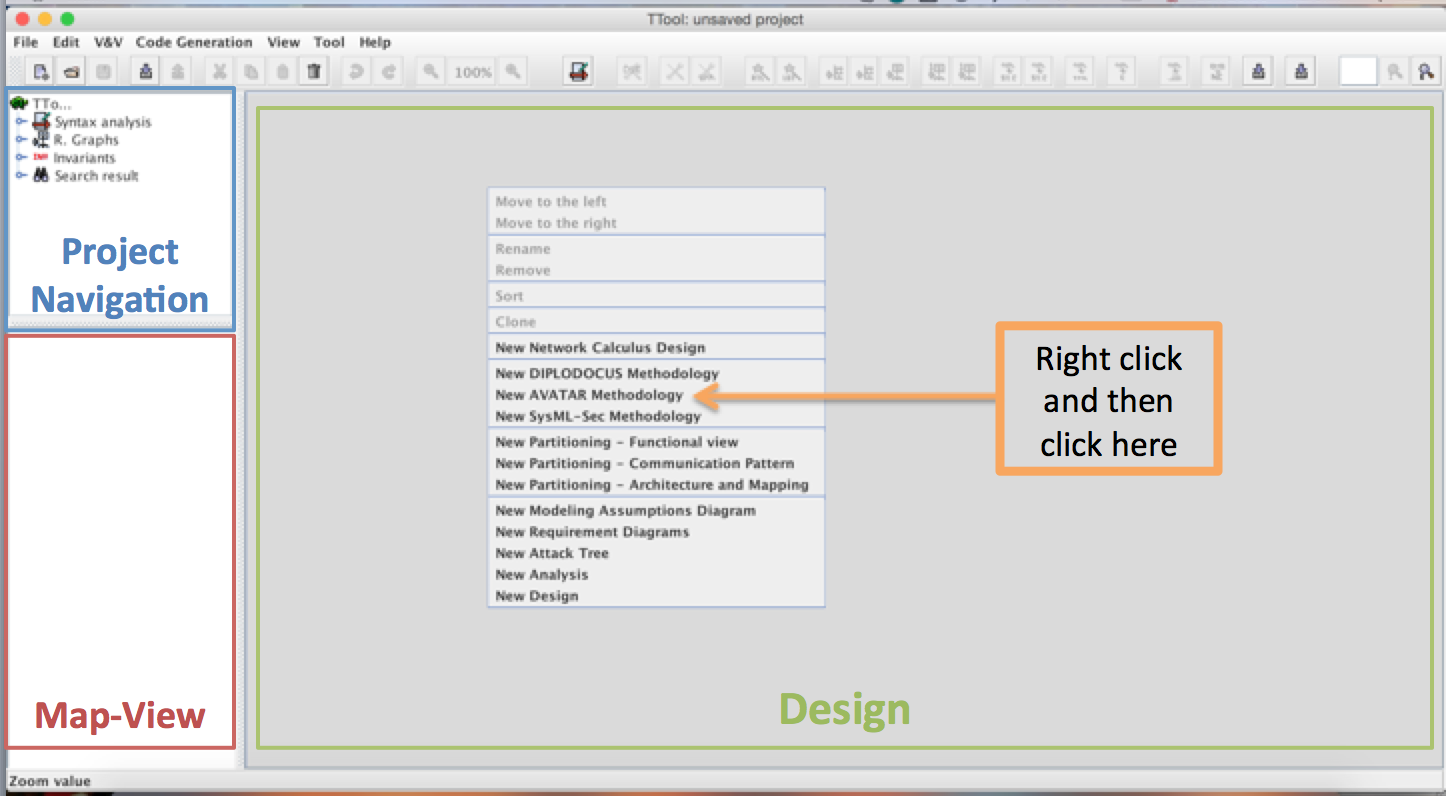
\includegraphics[width=0.99\textwidth]{fig/createmethod.png}
\caption{Create an AVATAR Methodology} \label{fig:createmethod}
\end{figure*}

To begin, we will start with the creation of a Methodology diagram as the one shown on Figure \ref{fig:methoddiagram}. In order to do this, right click on the design window and select “New AVATAR Methodology” (Figure \ref{fig:createmethod}). For each box on this diagram another diagram from the development of the project will be selected, however, this example will not include any properties or prototyping and therefore, these two boxes will remain blank. After all the other diagrams are created by following the steps in the remainder of this manual, one will go back to the methodology diagram, double click on each box, select the diagram corresponding to it and click on the arrow as shown in Figure \ref{fig:selectdiagram} in order to select it. 


\begin{figure*}[htbp]
\centering
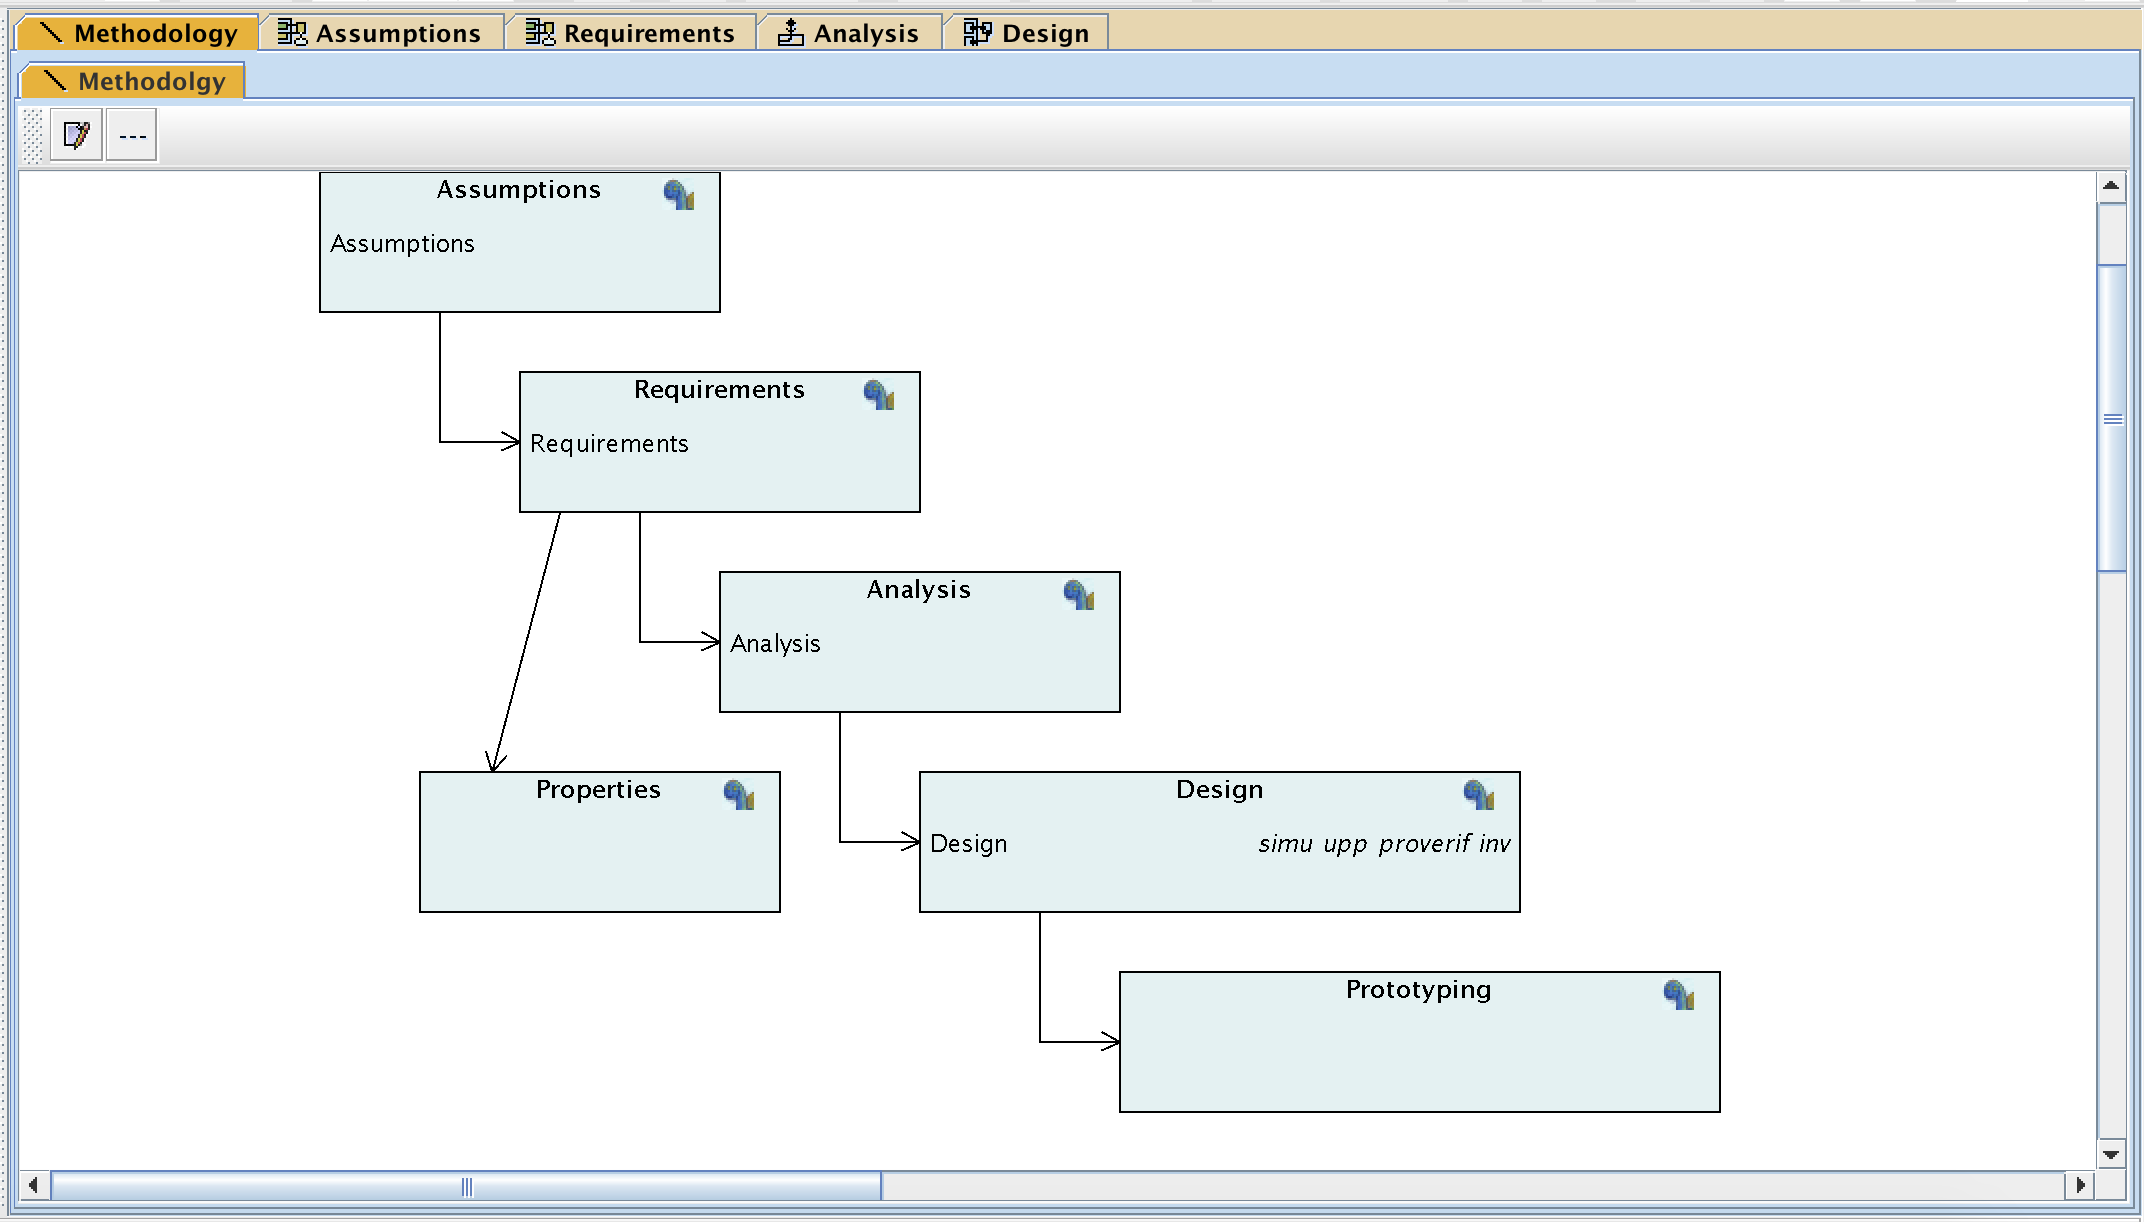
\includegraphics[width=0.99\textwidth]{fig/methoddiagram.png}
\caption{Methodology Diagram} \label{fig:methoddiagram}
\end{figure*}


\begin{figure*}[htbp]
\centering
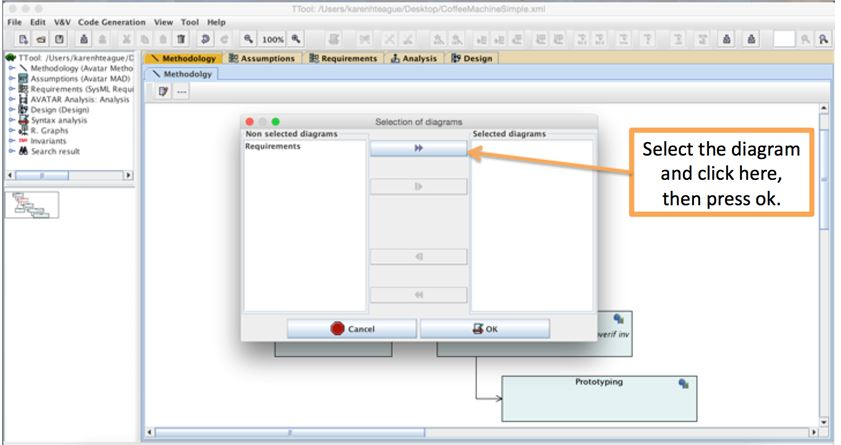
\includegraphics[width=0.99\textwidth]{fig/selectdiagram.jpg}
\caption{Selecting Diagrams} \label{fig:selectdiagram}
\end{figure*}


\section{Analysis}
\subsection{Assumptions}

As shown in Figure \ref{fig:assumptionswindow}, right click on the panel tab and add a “New Modeling Assumptions” diagram. By right clicking on the panel, it can be moved left or right. You will now have an Assumptions panel and underneath it an Assumptions diagram tab. You can right click on this tab in order to rename it, in this example, we changed its name to ‘System’. You will then add an assumption box by clicking on the AST button as shown in Figure \ref{fig:assumptionswindow}. You can add as many assumptions as needed in order to fully explain what is being taken into account for the system. 

\begin{figure*}[htbp]
\centering
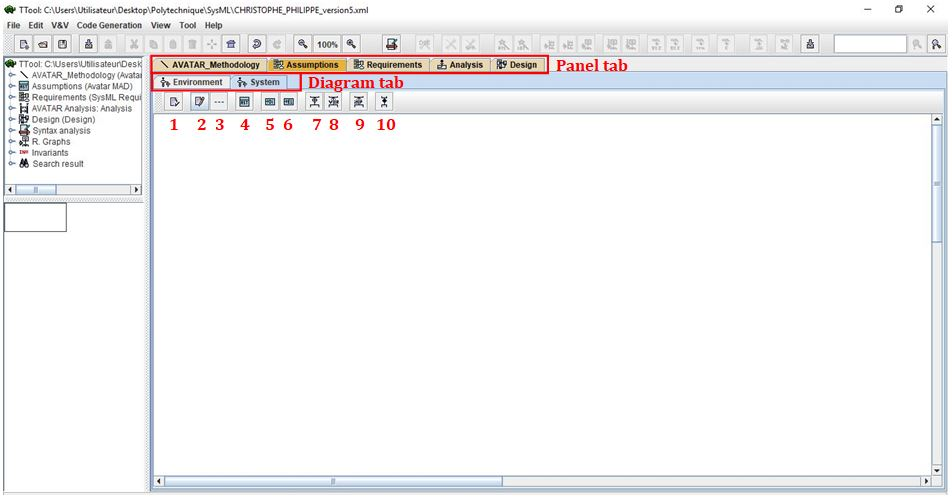
\includegraphics[width=0.99\textwidth]{fig/assumptionswindow.jpg}
\caption{Assumptions Window} \label{fig:assumptionswindow}
\end{figure*}

\begin{enumerate}
\item Edit AVATAR Modeling Assumptions Diagram
\item  Add a comment: add a comment to the diagram
\item  Comment connector
\item  AST: add an assumption box to the diagram
\item  Diagram reference: add a box who refers to another diagram
\item  Element reference: add a box who refers to an Avatar element
\item  Composite: Splits up a compound asuumptions into elementary ones
\item  Versioning: classify changes that are made to the original model
\item  Impact: indicate that the assumption at the origin of the link as a direct impact on the referenced element at the end on the link. 
\item Composition connector: relations between a diagram reference and elements references
\end{enumerate}

To edit each of these boxes, one should double click on them. A window like the one shown in Figure \ref{fig:assumptionsedit} will appear. In this window one can modify the name and type of the assumption, as well as other attributes such as durability, source, status and scope. Also, a little description of the assumption can be added in the box on the lower left corner. Furthermore, different types of links, or connections, can be added between the different boxes by clicking on the respective button shown in Figure \ref{fig:assumptionswindow} and then on the perimeter of each of the boxes you wish to link. 

\begin{figure*}[htbp]
\centering
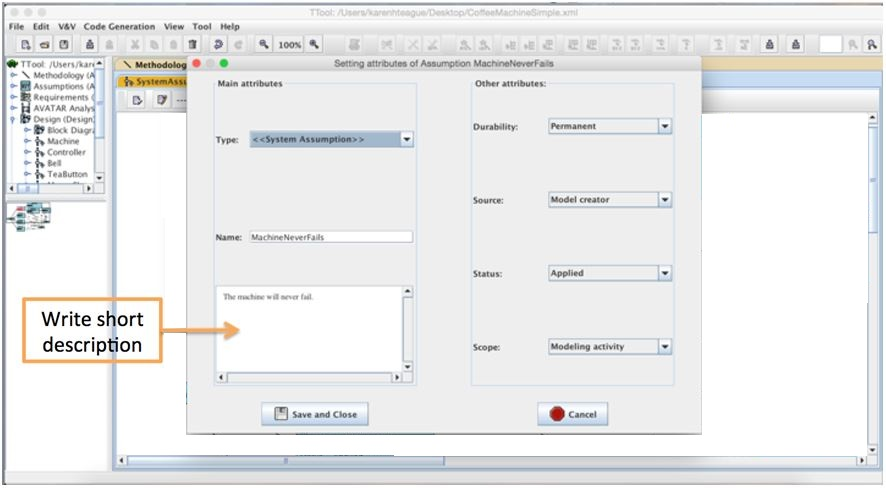
\includegraphics[width=0.99\textwidth]{fig/assumptionsedit.jpg}
\caption{Assumptions Editing} \label{fig:assumptionsedit}
\end{figure*}

Finally, in this example we have created two assumption diagrams; one for the system itself and one for the environment. The first one contains all the assumptions made directly about the system, while the second includes assumptions that may not be directly included in the system, but will affect its performance as shown in Figure \ref{fig:envassumptions}. One can add as many diagrams as one pleases by simply right clicking next to the existing diagram and selecting ``New AVATAR Modeling Assumptions Diagram'' and following the previously mentioned steps.

It is important to keep in mind that these assumptions will allow the creator and others needing to interact with the system to keep track of what was and was not considered during design. Therefore, one should attempt to be as descriptive as possible. This will make future improvements and changes easier while providing essential information about the system itself, resulting in a more complete design. 

As shown in Figure \ref{fig:systemassumptions}, the system assumptions made for the coffee machine are those who enable the system to perform without malfunction. For example, we have assumed the lack of failures due to power outages and connectivity failures. 

The environment assumptions were divided in two main categories: the sensors and the actuators. In this example, due to the short number of environment assumptions, they were all created on the same diagram as shown in Figure \ref{fig:envassumptions}. It should be noted that there could be three diagrams for the environment assumptions only. The first one would indicate the link between the environment and the two other diagrams, which would be the sensors diagram and the actuators diagram.
\begin{figure*}[htbp]
\centering
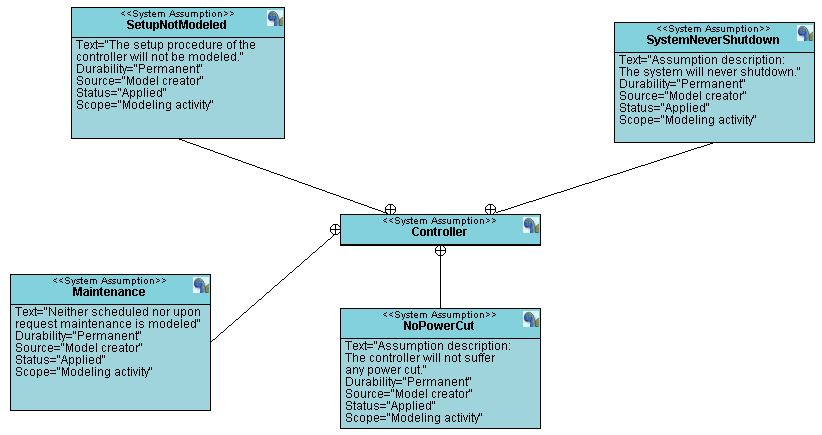
\includegraphics[width=0.99\textwidth]{fig/systemassumptions.jpg}
\caption{System Assumptions} \label{fig:systemassumptions}
\end{figure*}

The coffee machine has two type of sensors, a currency detector and pushbuttons. Together, they allow the users to order a cup of coffee or a cup of tea, and to pay for it. For their part, the actuators shall allow the users to receive their order. This part was fulfilled by the mechanical device. A mechanism permitting a transfer of information to the users was added to improve the ease of use of the coffee machine. As for the system, the assumptions enable the system to perform without malfunction.

\begin{figure*}[htbp]
\centering
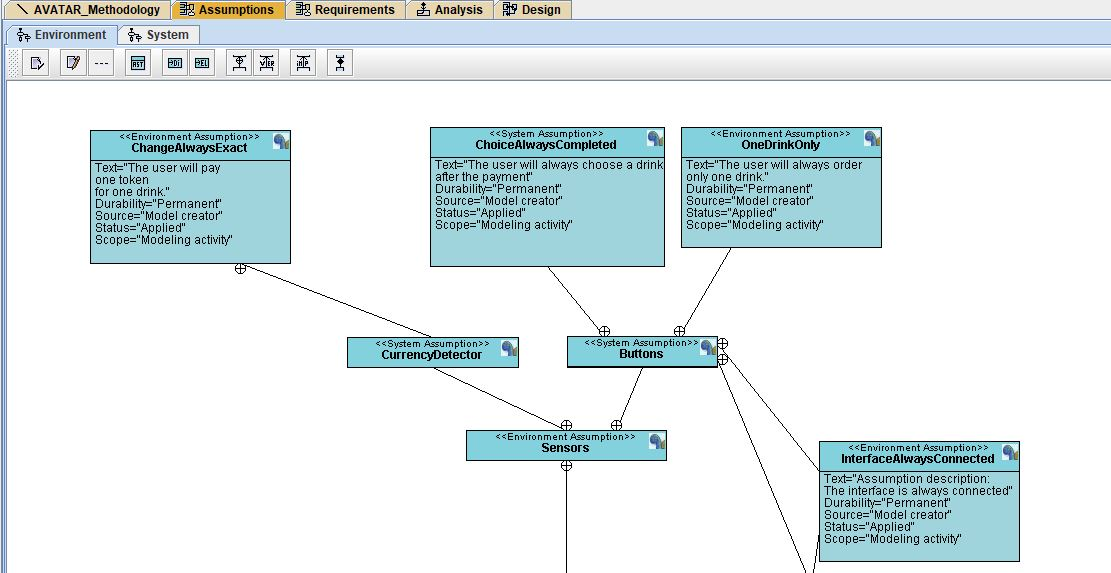
\includegraphics[width=0.99\textwidth]{fig/environmentassumptions.jpg}
\caption{Environment Assumptions} \label{fig:envassumptions}
\end{figure*}

\subsection{Requirements}
A requirement is a capability or a condition that the system must satisfy. It can be about a function that the system shall perform or a performance condition that must be achieved. Figure \ref{fig:reqbox} shows the standard form and information of a requirement box.

\begin{figure*}[htbp]
\centering
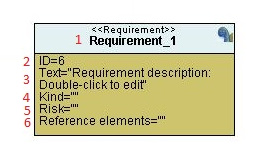
\includegraphics[width=0.3\textwidth]{fig/reqbox.jpg}
\caption{Requirement Box} \label{fig:reqbox}
\end{figure*}

\begin{itemize}
\item Requirement name
\item ID: unique identifier
\item Text: text requirement
\item Kind: status
\item Risk: priority
\item Reference elements
\end{itemize}

There are two parts where the requirements can be expressed. The use cases, which is a part of the analysis diagram, can be useful to express the functional requirements. However, it is not suitable for non-functional requirements. For its part, the requirements diagram enables us to introduce text-based requirements, providing a way to express the non-functional requirements. This diagram follows after setting up the assumptions for our system.

We will create one or several diagrams defining the requirements that the coffee machine controller will have. To do this, right click on the panel tab as before, but instead select “New Requirement Diagrams”. Just as before, a new diagram tab will appear underneath. Once again, this diagram tab can be renamed as preferred following the same steps we used in the assumption diagrams.
	
For the coffee machine, we will divide the requirements in three parts: the requirements related to the inputs, the control and the outputs.
The first diagram is named ``General Requirement Diagram''. It contains the link between the three parts mentioned above, which will all have their own requirements diagram. 
	
		Figure \ref{fig:reqdiagram} shows the structural elements available to build the requirements diagram.


\begin{figure*}[htbp]
\centering
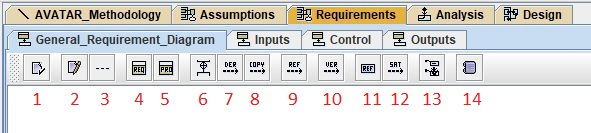
\includegraphics[width=0.7\textwidth]{fig/reqdiagram.jpg}
\caption{Structural elements of the requirements diagram} \label{fig:reqdiagram}
\end{figure*}

\begin{enumerate}
\item Edit Requirements Diagram
\item Add a comment: add a comment to the diagram
\item Comment connector
\item Requirement: add a requirement box to the diagram
\item Property: add a property box to the diagram
\item Composition: a relationship who defines the requirements hierarchy
\item DeriveReqt: a relationship who links two requirements of the same hierarchy but at different levels of abstraction
\item Copy: a relationship that connect a slave requirement a master requirement
\item Refine: a relationship who links used between a requirement that refine another
\item Verify: a relationship who defines how a model element verifies a requirement
\item Element reference
\item Satisfy: a relationship who show that a concept satisfies a requirement
\item Show/hide element attributes
\item Enhance

\end{enumerate}

Figure \ref{fig:reqgeneral} represents the general requirement diagram obtained for the coffee machine controller.

\begin{figure*}[htbp]
\centering
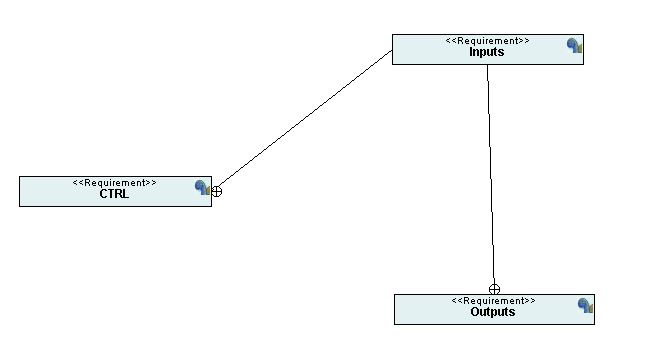
\includegraphics[width=0.99\textwidth]{fig/reqgeneral.jpg}
\caption{General Requirement Diagram} \label{fig:reqgeneral}
\end{figure*}


In a similar way to that of the assumptions, a new requirement can be added by selecting the requirement button shown in Figure \ref{fig:reqdiagram}. Once created, it can also be modified by double clicking on it. When the new window pops up, one can provide a description and change the ID, Type, Risk and Reference attributes of each requirement.
	The next step was to create the inputs diagram, the control diagram and the outputs diagram. By using the requirement box and relationships described in Figure \ref{fig:reqdiagram}, we obtained the diagrams shown in Figures \ref{fig:inputreq} and \ref{fig:controlreq}. 

\begin{figure*}[htbp]
\centering
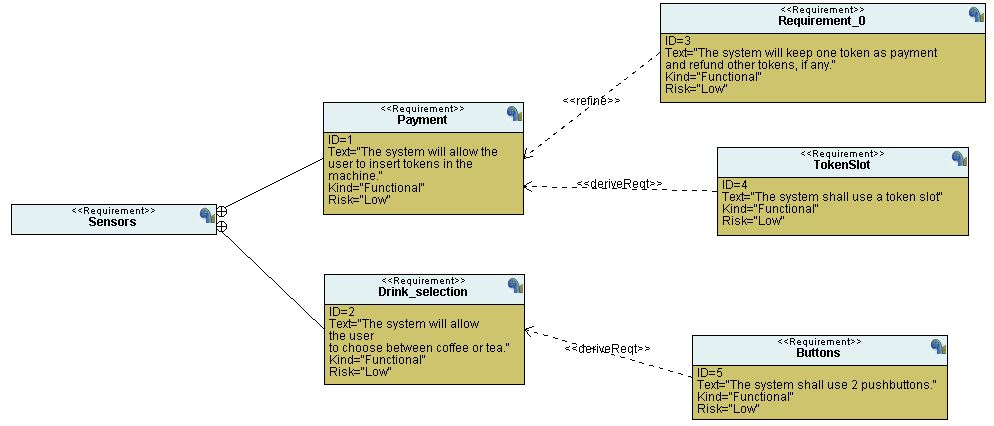
\includegraphics[width=0.99\textwidth]{fig/inputreq.jpg}
\caption{Inputs requirements diagram} \label{fig:inputreq}
\end{figure*}

\begin{figure*}[htbp]
\centering
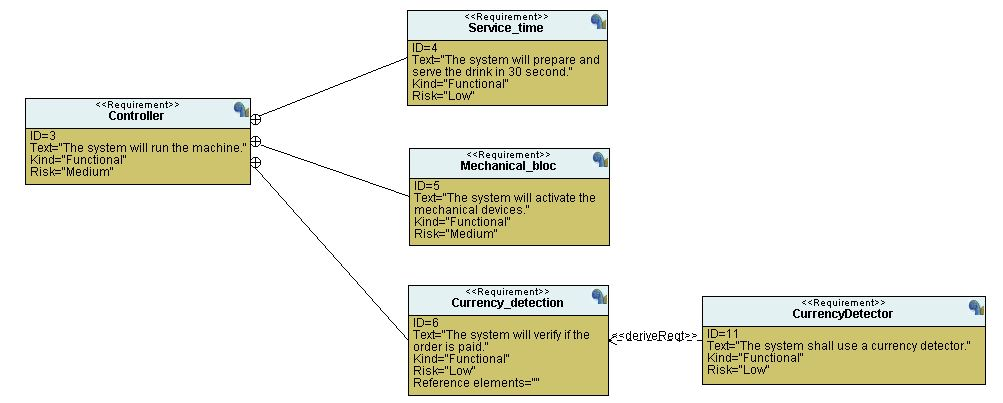
\includegraphics[width=0.99\textwidth]{fig/controlreq.jpg}
\caption{Control requirements diagram} \label{fig:controlreq}
\end{figure*}

\begin{figure*}[htbp]
\centering
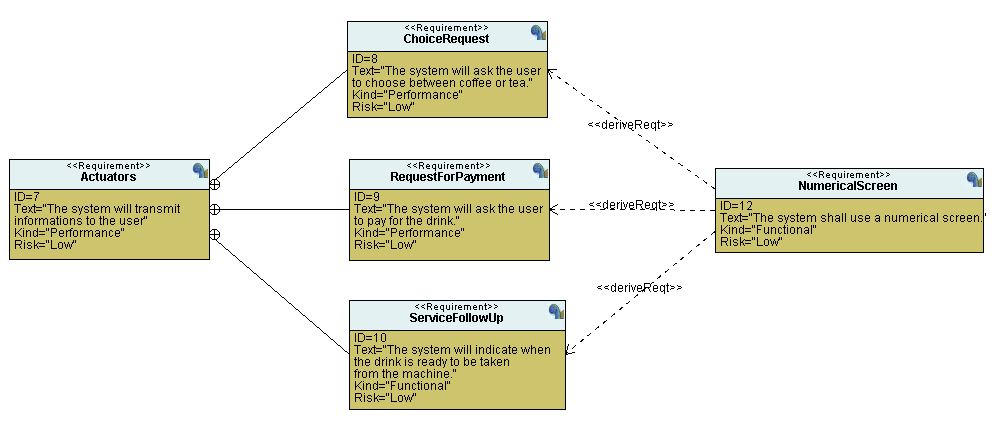
\includegraphics[width=0.99\textwidth]{fig/outputreq.jpg}
\caption{Output requirements diagram} \label{fig:outputreq}
\end{figure*}

\subsection{Use Case}
	Once again, right click on the panel tab. This time, select the “New Analysis” option, which will give you a window like the one shown in Figure \ref{fig:createusecase}. We will begin the analysis process with a Use Case Diagram. To add it, right click on the window and select “New Use Case Diagram”. This diagram will allow us to represent the system, the actors acting on it and the different instances or use cases that will be modeled. All these elements can be observed in Figure \ref{fig:usecase}. To add each of them you should use the buttons shown in Figure \ref{fig:structusecase}. To change the names, double click on each on them.
	
\begin{figure*}[htbp]
\centering
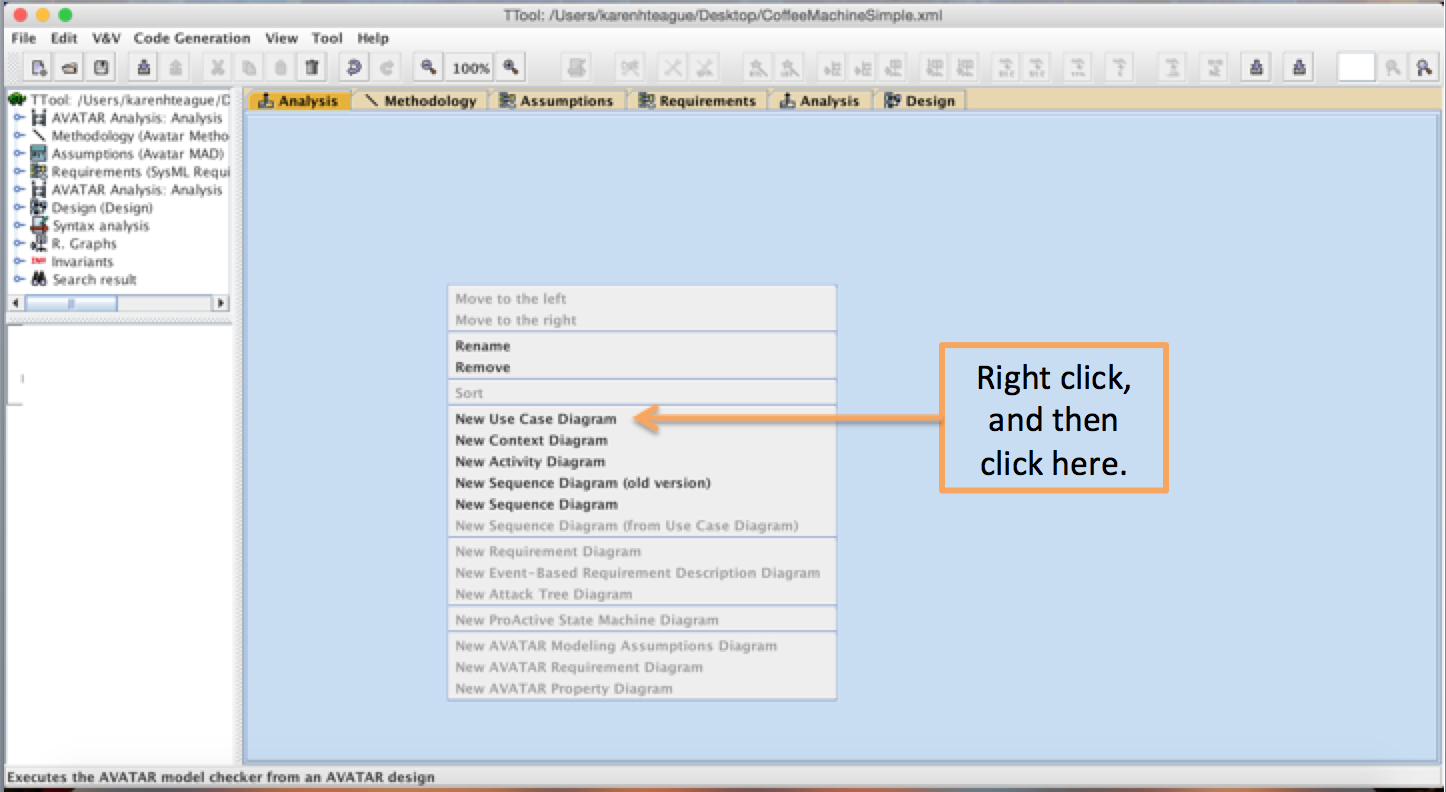
\includegraphics[width=0.99\textwidth]{fig/createusecase.png}
\caption{Create Use Case Diagram} \label{fig:createusecase}
\end{figure*}

\begin{figure*}[htbp]
\centering
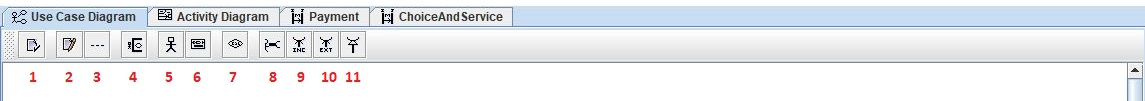
\includegraphics[width=0.99\textwidth]{fig/structusecase.jpg}
\caption{Structural elements of the use case diagram} \label{fig:structusecase}
\end{figure*}

\begin{figure*}[htbp]
\centering
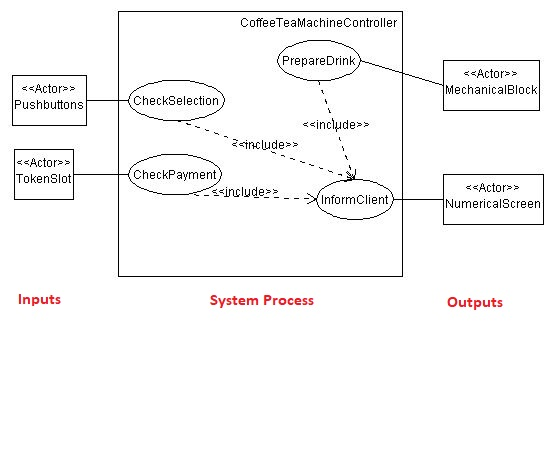
\includegraphics[width=0.99\textwidth]{fig/usecase.jpg}
\caption{Use Case Diagram} \label{fig:usecase}
\end{figure*}



\begin{enumerate}
\item Edit Use Case Diagram
\item Add a comment: add a comment to the diagram
\item Comment connector
\item Add a border: create a system box who defines the boundaries of the system
\item Actor: add an actor to the diagram
\item Actor (Box Format): add an actor box to the diagram
\item Add a use case
\item Actor <->use case: links an actor to a use case
\item Include: a relationship who links a function to a subfunction whose mandatorily included
\item Extend: a relationship who links a function to a sibfunction whose optionally included
\item Specialization: links a `parent' function whose specialized by a `child' function
\end{enumerate}

As shown in Figure \ref{fig:usecase}, on the left hand of the diagram, one can find the actors that initialize a process, while on the right we have the actors or elements that are activated as a result of it. The box in the middle represents the enclosed system and the four bubbles inside of it are the use cases: they represent the actions that the system will perform and are linked to the actor(s) involved in them. The links are usually an action description in a few words.

Once done, the next step is to create an activity diagram. Just as before, right click on the diagram tab and select “New Activity Diagram”.  In TTool, an activity diagram is portrayed in the form of what is commonly known as a flowchart. The elements that can be added to it are shown on the button tab and they include activities, partitions, the start and end of the activity, choices and tabs for whether there is a signal being sent or received. 

\begin{figure*}[htbp]
\centering
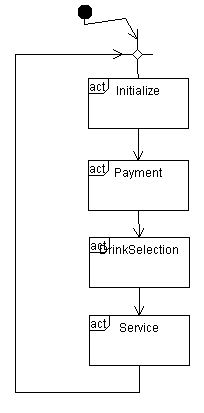
\includegraphics[width=0.4\textwidth]{fig/actdiagram.jpg}
\caption{Activity Diagram} \label{fig:actdiagram}
\end{figure*}
 
In the example shown in Figure \ref{fig:actdiagram}, only a start, activities and a junction are used.  After each of the elements is added, they can be edited by double clicking on them. The activity boxes should represent each of the steps that the system will perform. In addition, to edit the choice elements, click on each of the brackets or guards that appear on each of the rhombus connectors and write in the condition that must be satisfied for each option. Finally, the arrows, or associations, can be added by clicking on the respective button and then by clicking on a point on the perimeter of each of the elements being linked.
	The final section of the analysis is creating a scenario or sequence. As in previous, cases right click on the diagram tab and select “New Sequence Diagram.” This diagram will allow us to showcase the logical progression of actions as well as the different instances in which different actors or components come into play during the execution of the system. Using the different buttons at the top of the window one can add instances, timers and indicate whether the message being transmitted is synchronous or asynchronous1 among other elements. 
To add an actor, click the “Instance” button and place it on the window. Then, double click as if to edit. When the pop up window appears, check the box that says “actor”. After setting up the main structure of the system use the arrows mentioned before to represent the messages being sent between the different elements, add text describing the process by double clicking on them after setting them in place. Though not shown in this example, when adding a timer one must also indicate the amount of time assigned to it and its attributes.

As shown in Figure \ref{fig:paymentseqdiagram} and \ref{fig:choiceseqdiagram}, the sequence diagram functions as a visual description of the flow of messages and information inside the system. If required, one can create more than one diagram in the same window, or add as many sequence diagrams as necessary.

\begin{figure*}[htbp]
\centering
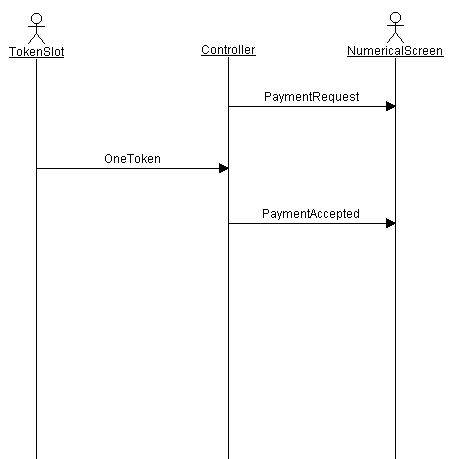
\includegraphics[width=0.99\textwidth]{fig/paymentseqdiagram.jpg}
\caption{Logical progession of the `Payment' sequence diagram} \label{fig:paymentseqdiagram}
\end{figure*}

\begin{figure*}[htbp]
\centering
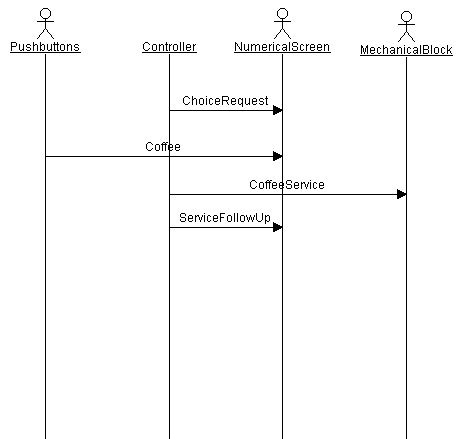
\includegraphics[width=0.99\textwidth]{fig/choiceseqdiagram.jpg}
\caption{Logical progression of the `ChoiceAndService' sequence diagram} \label{fig:choiceseqdiagram}
\end{figure*}

\section{Design}
	Just as with all the previous sections, to start the design, one will right click on the panel tab and select “New Design”. This will open the window to create a “Block Diagram”-- here we will create the main structure of our system. To add a block, click on the block button shown in Figure \ref{fig:blockdiagram}. You will create as many blocks as actors/parts you have determined in the previous parts of the creation process. 


\begin{figure*}[htbp]
\centering
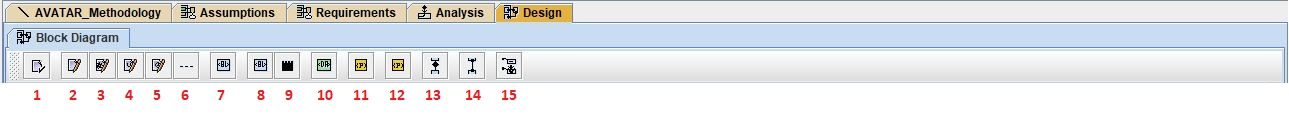
\includegraphics[width=0.99\textwidth]{fig/blockdiagram.jpg}
\caption{Structural elements of the block diagram} \label{fig:blockdiagram}
\end{figure*}


\begin{enumerate}
\item Edit interaction overview diagram
\item Add a comment: add a comment to the diagram
\item Security pragmas
\item Safety property
\item Performance property
\item Comment connector
\item Block
\item Crypto block
\item Add an avatar firewall
\item Data type 
\item Library function
\item Crypto library function
\item Composition connector
\item Port connector
\item Show/hide element attributes

\end{enumerate}

The coffee machine controller has five blocks: the pushbuttons, the token slot, the controller of the machine, the mechanical block, and the numerical screen. The name of each block can be edited by double clicking on the top part of the block and writing in the desired name. In addition, every time a block is created, a new tab corresponding to that block will appear next to the block diagram. We will look further into each of them later in this manual.

	Following the creation of the blocks, attributes and signals for each of them will be added. To do this, double click on the bottom part of the block. A pop up window as the one shown in Figure \ref{fig:setattribute} will show up. In the ‘Attributes’ section we will indicate the elements or variables that will interact with that section of the machine and whether they are integers, timer or Boolean values. In this example only the token slot, the controller and the pushbuttons have ‘Attributes’. In the two first of them we can find “T” (short for token), which is an integer. This can be defined by selecting “int” from the drop down menu in the section indicated in Figure \ref{fig:setattribute}. In addition, in the two last of them we can find timers.


\begin{figure*}[htbp]
\centering
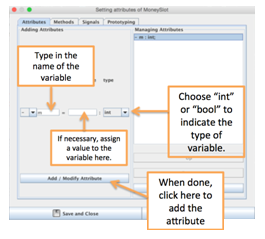
\includegraphics[width=0.5\textwidth]{fig/setattribute.png}
\caption{Setting attributes of a block} \label{fig:setattribute}
\end{figure*}


Furthermore, the ‘signals’ represent the information being sent and received by each component of the machine. On the same pop up window as before, click on the signals tab on the top. To add a signal, just select whether it is coming in or going out in the box shown in Figure \ref{fig:setsignal} and then give it a name. If two blocks have communication between them, one should have the outgoing signal, and the other the receiving signal. 

\begin{figure*}[htbp]
\centering
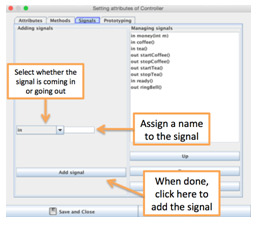
\includegraphics[width=0.5\textwidth]{fig/setsignal.png}
\caption{Setting signals of a block} \label{fig:setsignal}
\end{figure*}


	Finally, one will add port connections by clicking on the respective button shown in Figure \ref{fig:blockdiagram}, and then selecting a point on the perimeter of the blocks being connected. Next, double click on the connector; a new window will pop up (Figure \ref{fig:portconn}). 
	
	\begin{figure*}[htbp]
\centering
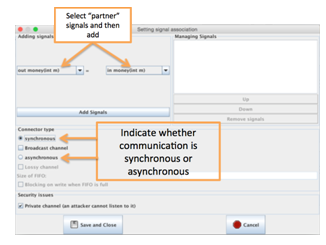
\includegraphics[width=0.5\textwidth]{fig/portconn.png}
\caption{Port Connection between blocks} \label{fig:portconn}
\end{figure*}

	Here you will select the outgoing and incoming pairs of signals and one by one add them as shown in Figure \ref{fig:portconn}. In addition, you can select whether this message is asynchronous or synchronous on the boxes in the inferior part of the window. Once all the signals and connections between each of the blocks are set, we can move on to the diagrams for each of the blocks.
The block diagram created for the coffee machine controller is shown in Figure \ref{fig:blockdiag}.

	\begin{figure*}[htbp]
\centering
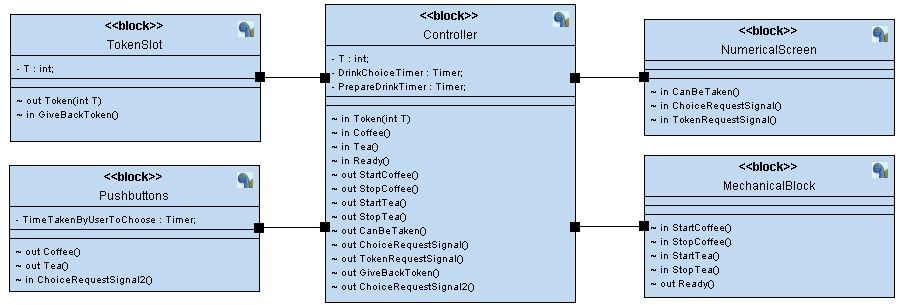
\includegraphics[width=0.99\textwidth]{fig/blockdiag.jpg}
\caption{Block diagram} \label{fig:blockdiag}
\end{figure*}

Once the block diagram is finished, we will go to the tabs that appeared for each of the blocks. Here, we will show through a flow chart the process through which each element goes to complete its specified task. Unlike before, in this case the black dot that indicates the process is starting is automatically added. We will complete the design from there down. Also, differently than in the activity diagram created during the analysis, here we can add the states in which the machine, or part of the machine is, choices, signals being sent and received and stops. Each of these buttons are shown in Figure \ref{fig:structelementsblock}. 

\begin{figure*}[htbp]
\centering
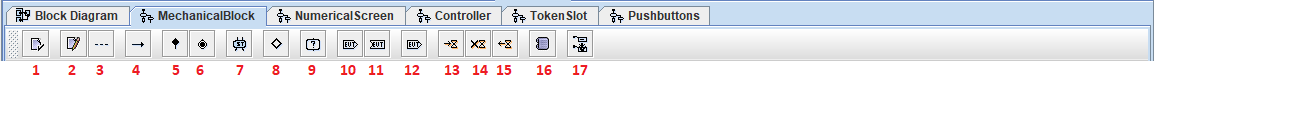
\includegraphics[width=0.99\textwidth]{fig/structelementsblock.png}
\caption{Structural elements of each block diagram} \label{fig:structelementsblock}
\end{figure*}

\begin{enumerate}
\item Edit AVATAR state machine diagram
\item Add a comment: add a comment to the diagram
\item Comment connector
\item Connect two operators together
\item Start: add a starting point to the diagram
\item Stop: add a stopping point which will be the final state when it is reached (the block instance `dies')
\item State
\item Choice: add transitions that can be taken following specific conditions
\item Select random: add an attribute that can give a random value to a variable
\item Send signal: add an output signal
\item Receive signal: add an input signal
\item Library function call
\item Set timer: add a timer that will start when it is reached
\item Reset timer: stop the timer's clock and reset it
\item Wait for timer expiration
\item Enhance
\item Show/hide AVATAR IDs
\end{enumerate}

Using as reference what was already indicated in the block diagram, we will determine when messages are being sent and the states in which the machine is before and after each iteration. The diagrams for the mechanical block, numerical screen, controller, token slot and pushbuttons can be observed as example in Figures \ref{fig:mechdiagram} to \ref{fig:pushbuttondiagram} respectively.
\begin{figure*}[htbp]
\centering
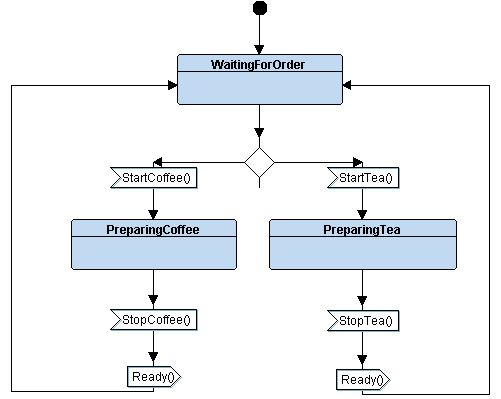
\includegraphics[width=0.99\textwidth]{fig/mechdiagram.jpg}
\caption{Mechanical block diagram} \label{fig:mechdiagram}
\end{figure*}

\begin{figure*}[htbp]
\centering
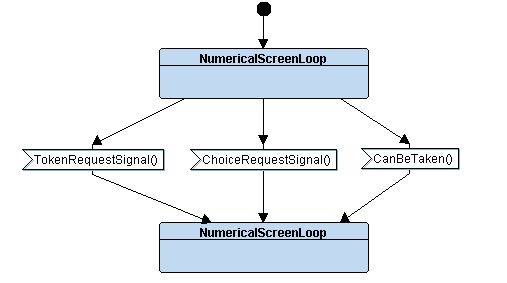
\includegraphics[width=0.99\textwidth]{fig/numdiagram.jpg}
\caption{Numerical screen diagram} \label{fig:numdiagram}
\end{figure*}

\begin{figure*}[htbp]
\centering
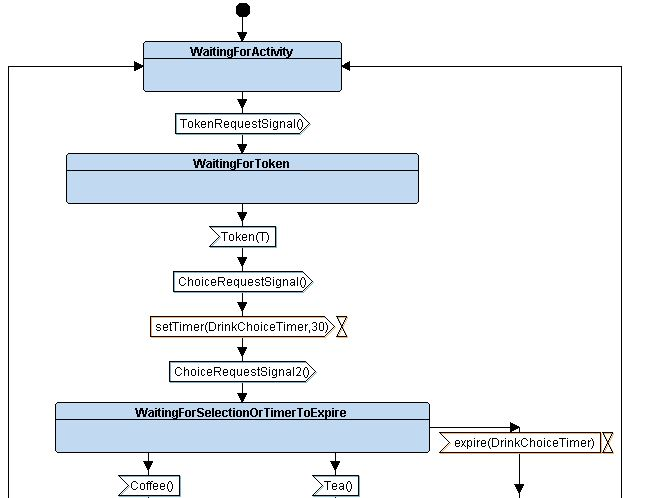
\includegraphics[width=0.99\textwidth]{fig/controllerdiagram.jpg}
\caption{Controller diagram} \label{fig:controllerdiagram}
\end{figure*}

\begin{figure*}[htbp]
\centering
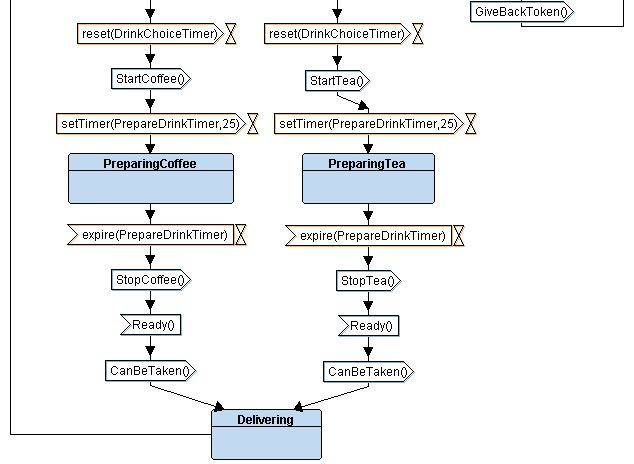
\includegraphics[width=0.9\textwidth]{fig/tokendiagram.jpg}
\caption{Token slot diagram} \label{fig:tokendiagram}
\end{figure*}

\begin{figure*}[htbp]
\centering
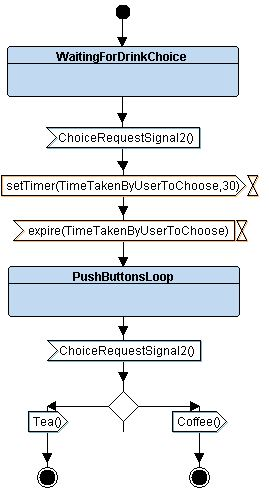
\includegraphics[width=0.5\textwidth]{fig/pushdiagram.jpg}
\caption{Pushbuttons diagram} \label{fig:pushbuttondiagram}
\end{figure*}

\section{Verification}
	Finally, the last step of the process is to verify that the system we have created works properly and follows each of the steps we desire it to. In order to do this, we will use the “Syntax Analysis” tool, which is shown in Figure \ref{fig:syntaxanalysis}. After you click on it, a screen like the one in this same figure will appear. There you can select whether you want to check the syntax of the whole system or individual parts. After this is determined, click on start syntax analysis and wait a second. After the software is done, it will either pop up an error message like the one in Figure \ref{fig:syntaxerror}, meaning that the system has not been designed correctly; or if no errors are found, the “Interactive Simulation” button (Figure \ref{fig:syntaxanalysis}), which was once greyed out, will now be blue and you will be able to click on it.

\begin{enumerate}
\item Syntax Analysis
\item Select elements to analyze
\item Start analysis
\item Interactive Simulation (currently greyed out)


\end{enumerate}
\begin{figure*}[htbp]
\centering
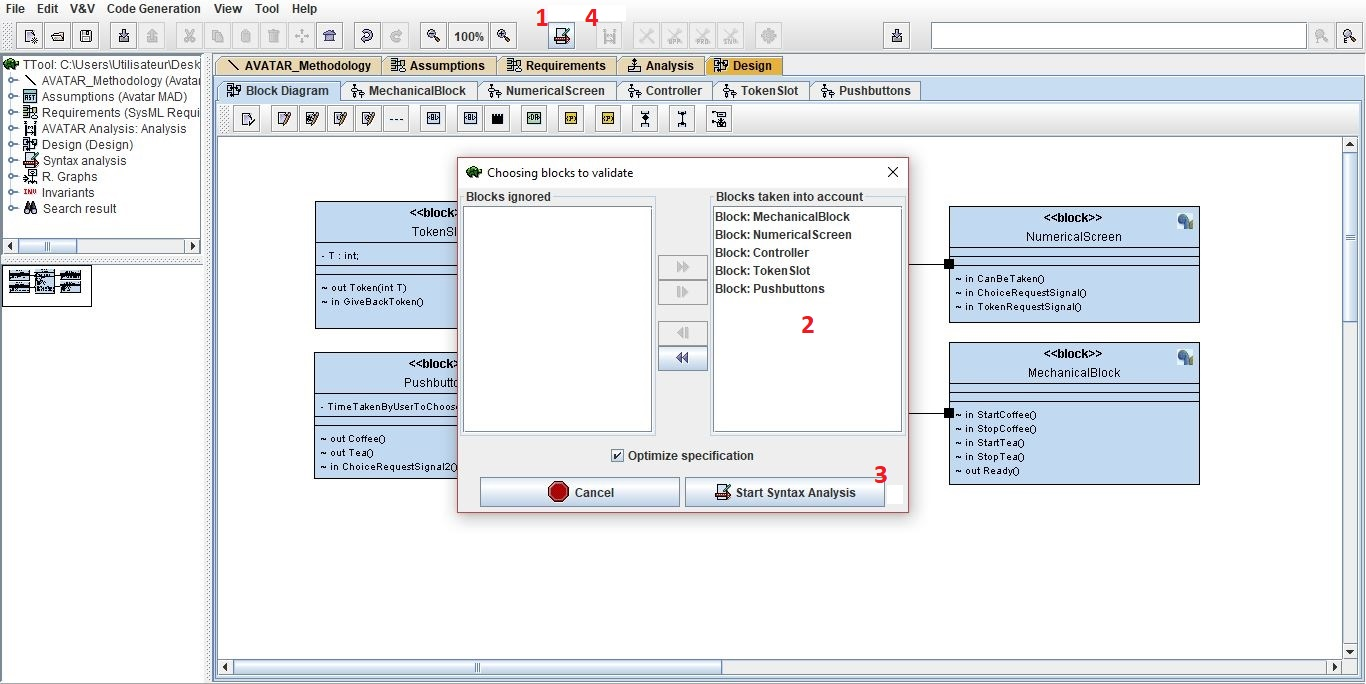
\includegraphics[width=0.99\textwidth]{fig/syntaxanalysis.jpg}
\caption{Syntax analysis} \label{fig:syntaxanalysis}
\end{figure*}


\begin{figure*}[htbp]
\centering
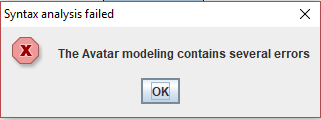
\includegraphics[width=0.3\textwidth]{fig/syntaxerror.png}
\caption{Syntax analysis error message} \label{fig:syntaxerror}
\end{figure*}

	If this is the case, then you will click on it and a window like the one in Figure \ref{fig:interactivesim} will appear on your screen. Click on run simulation and wait. The software will then go through a full iteration of the machine and show each step in the way portrayed by Figures \ref{fig:simstep1} and \ref{fig:simstep2} below. This tool is very useful in that it allows us to see how the different parts of the machine communicate as well as each step of the process programmed.
\subsection{Reachability Graphs}

\begin{figure*}[htbp]
\centering
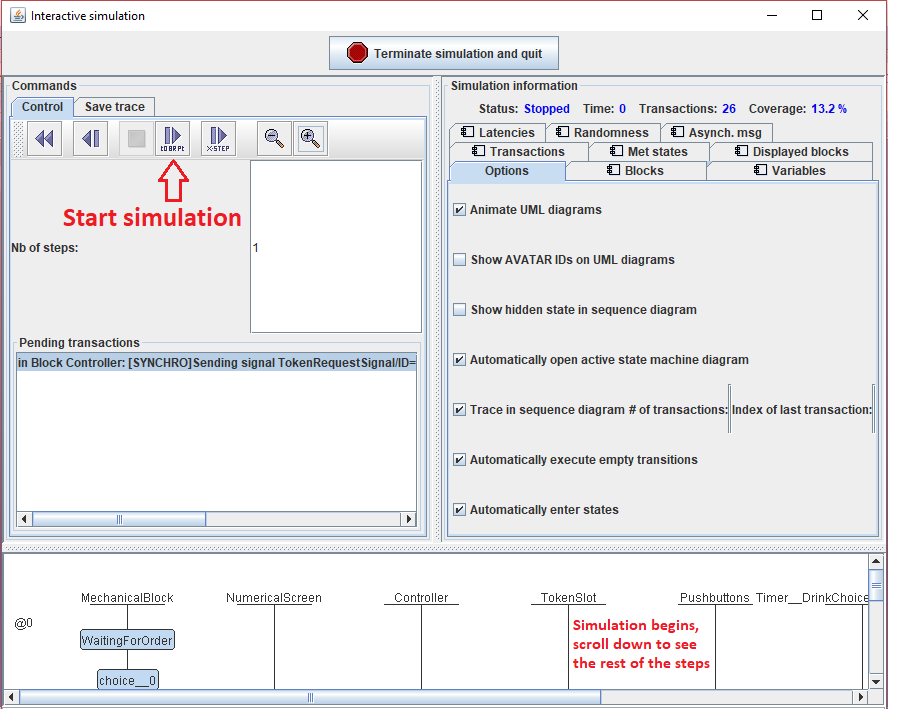
\includegraphics[width=0.99\textwidth]{fig/interactivesim.png}
\caption{Interactive Simulation} \label{fig:interactivesim}
\end{figure*}

\begin{figure*}[htbp]
\centering
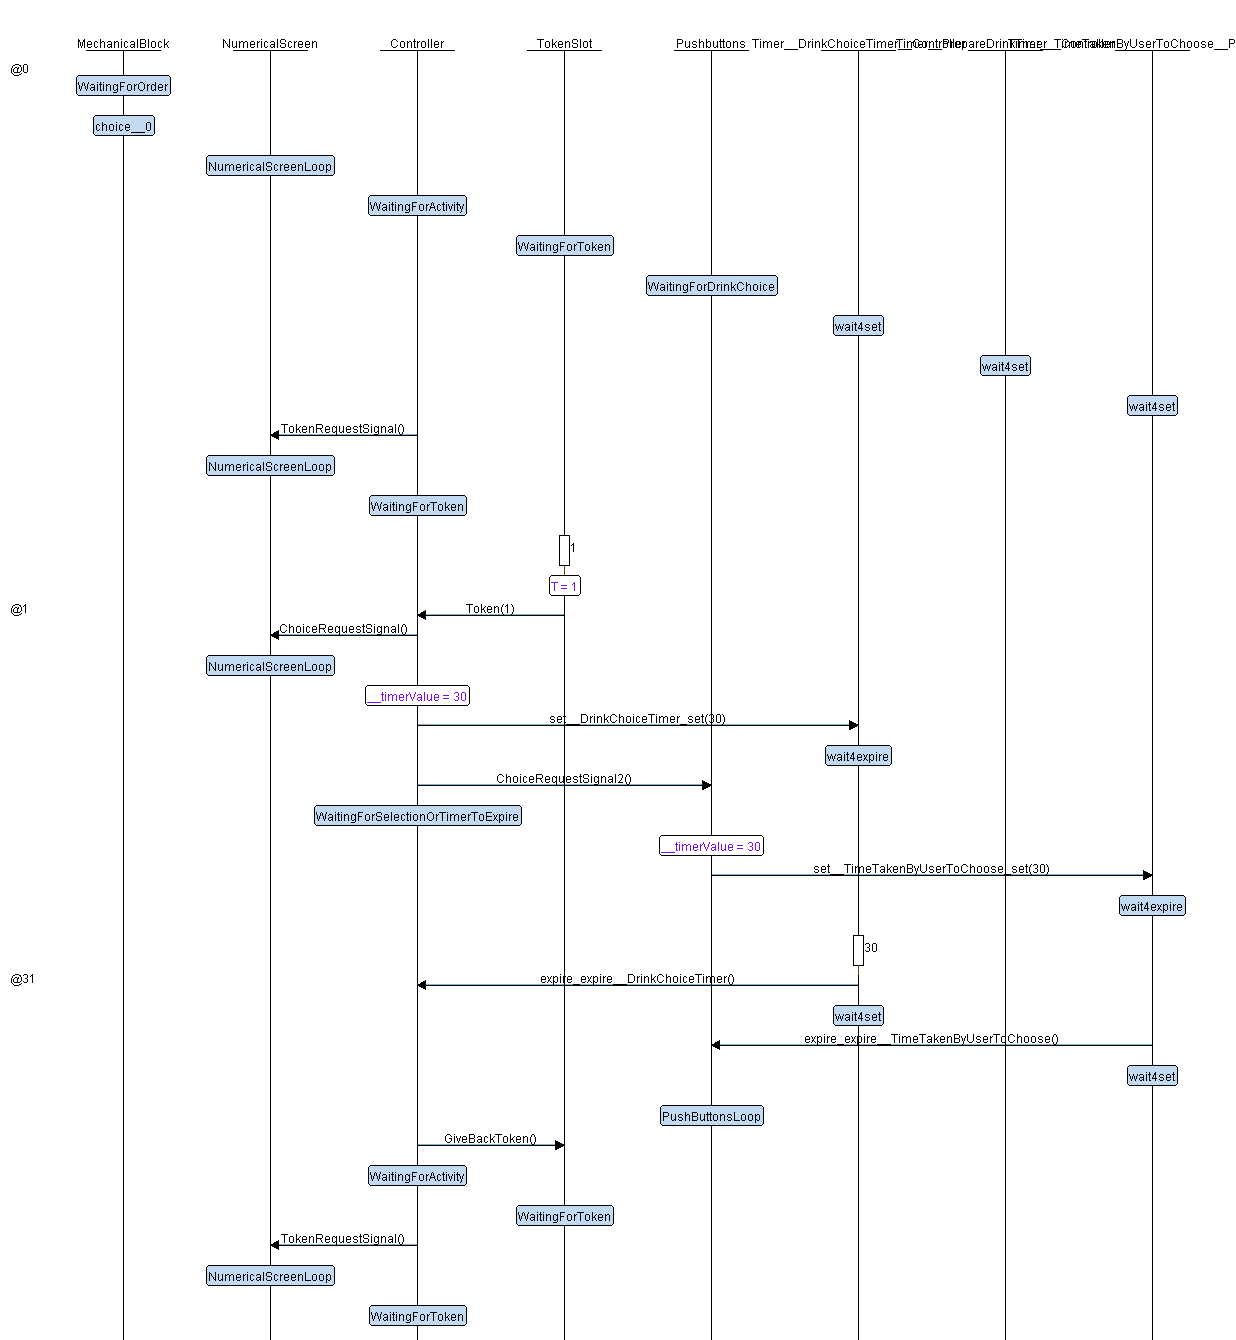
\includegraphics[width=0.99\textwidth]{fig/simstep1.png}
\caption{Simulation steps (part 1)} \label{fig:simstep1}
\end{figure*}

\begin{figure*}[htbp]
\centering
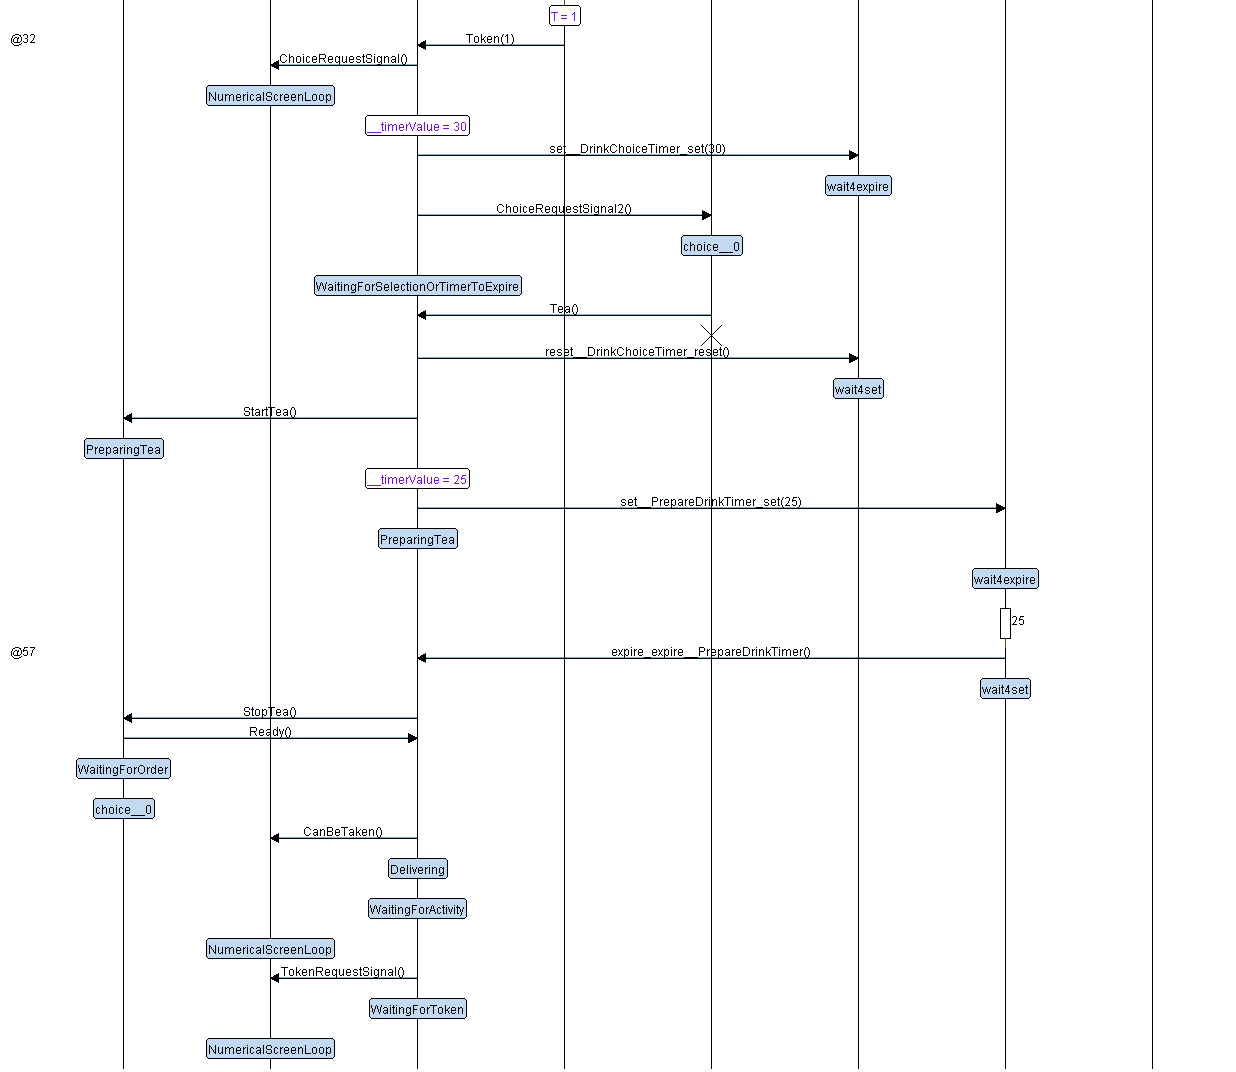
\includegraphics[width=0.99\textwidth]{fig/simstep2.png}
\caption{Simulation steps (part 2)} \label{fig:simstep2}
\end{figure*}


	Another interesting feature in the TTool software is the ability to graph or map the processes. This generates a graph that allows us to see all the different pathways that the system follows to reach its final state, each showing a different scenario. In addition, one can select a specific initial and final state, which simplifies said graph and gives a neater depiction of the process. Figure \ref{fig:rg} shows an example. 

\begin{figure*}[htbp]
\centering
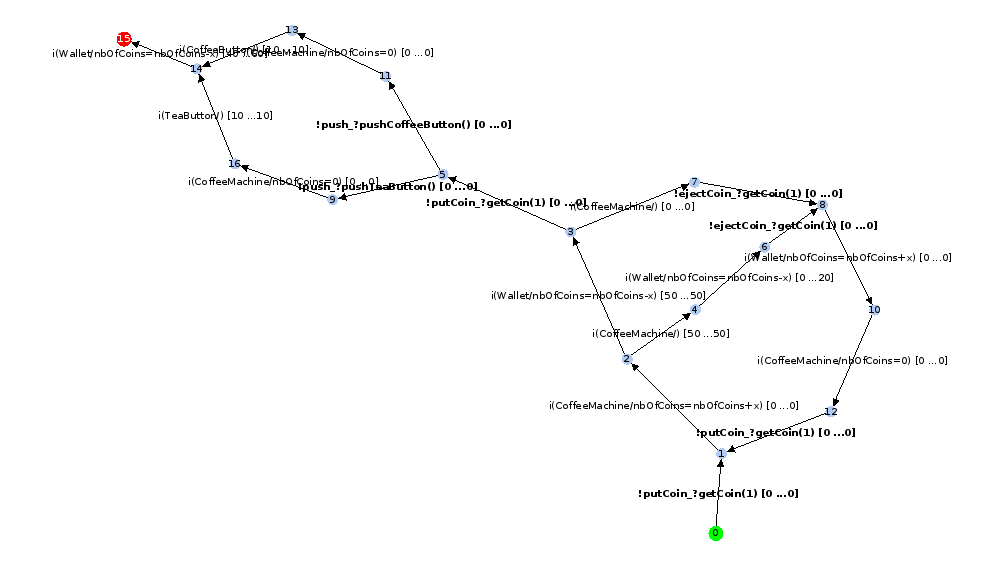
\includegraphics[width=0.99\textwidth]{fig/rg.png}
\caption{Reachability graph} \label{fig:rg}
\end{figure*}

\subsection{Safety pragmas}
Safety pragmas can be inserted in the model. These pragmas follow the following grammar.

\setlength{\grammarparsep}{20pt plus 1pt minus 1pt} % increase separation between rules
\setlength{\grammarindent}{12em} % increase separation between LHS/RHS 

\begin{grammar}

<pragma> ::= <path> <state> <property> 
\alt <property> <leadsto> <property> 

<path> ::=  `A'  |   `E' 

<state> ::=  `<>'  |   `[]' 

<leadsto> ::=  `-->'  

<property> ::= <stateproperty>
\alt <intproperty>
\alt <boolproperty>
\alt <property> <binaryop> <property>

<stateproperty> ::= `BlockName.stateName' 

<intproperty> ::= <intexpr> <intcomparator> <intexpr>

<boolproperty> ::= <boolexpr> <boolcomparator> <boolexpr>
\alt <boolexpr>



<intexpr> ::= `BlockName.integerattribute' 
\alt <intvalue>

<intexpr> ::= `BlockName.booleanattribute' 
\alt <booleanvalue>


<binaryop>  ::=  `&&'  |   `||' 

<intvalue> :: <integer>

<booleanvalue> :: `true' | `false'

<intcomparator>  ::=  `<'  |   `>'  | `=='  |   `!=' 

<boolcomparator> ::=  `=='  |   `!=' 

\end{grammar}

\subsection{Latency Analysis}


Many real-time safety-critical systems interact continuously with the environment and users. New input from the outside world is processed by the system, which then effectuates a response observable in the real world. The timing of such responses can greatly impact functionality and safety.

Latency analysis is performed in multiple steps. First, the quantitative requirement on latency must be defined. Next, the text requirement must be translated to determine which modeling elements the critical events refer to, after which latencies can be measured in simulation. The results are then conveniently displayed on the modeling diagrams. This example uses the updated Coffee Machine model that can be found in the TTool sample modeling repository.

Figure \ref{fig:latencyreq} shows a requirement related to timing: The Coffee Machine must take less than X seconds to finish a drink command after payment has been received. 

\begin{figure*}[htbp]
\centering
\includegraphics[width=0.3\textwidth]{build/latencyreq-svg.pdf}
\caption{Latency Requirement for Coffee Machine} \label{fig:latencyreq}
\end{figure*}

The operators relating to this requirement are the last `getCoin(x)' and the idle state after processing `WaitingForFirstCoin'. Figure \ref{fig:latencycheckpoint} shows how the two operators are tagged with `Latency Checkpoints', in the form of blue flags.

\begin{figure*}[htbp]
\centering
\includegraphics[width=0.99\textwidth]{build/latencycheckpoint-svg.pdf}
\caption{Latency Checkpoints in State Machine Diagrams} \label{fig:latencycheckpoint}
\end{figure*}


\begin{figure*}[htbp]
\centering
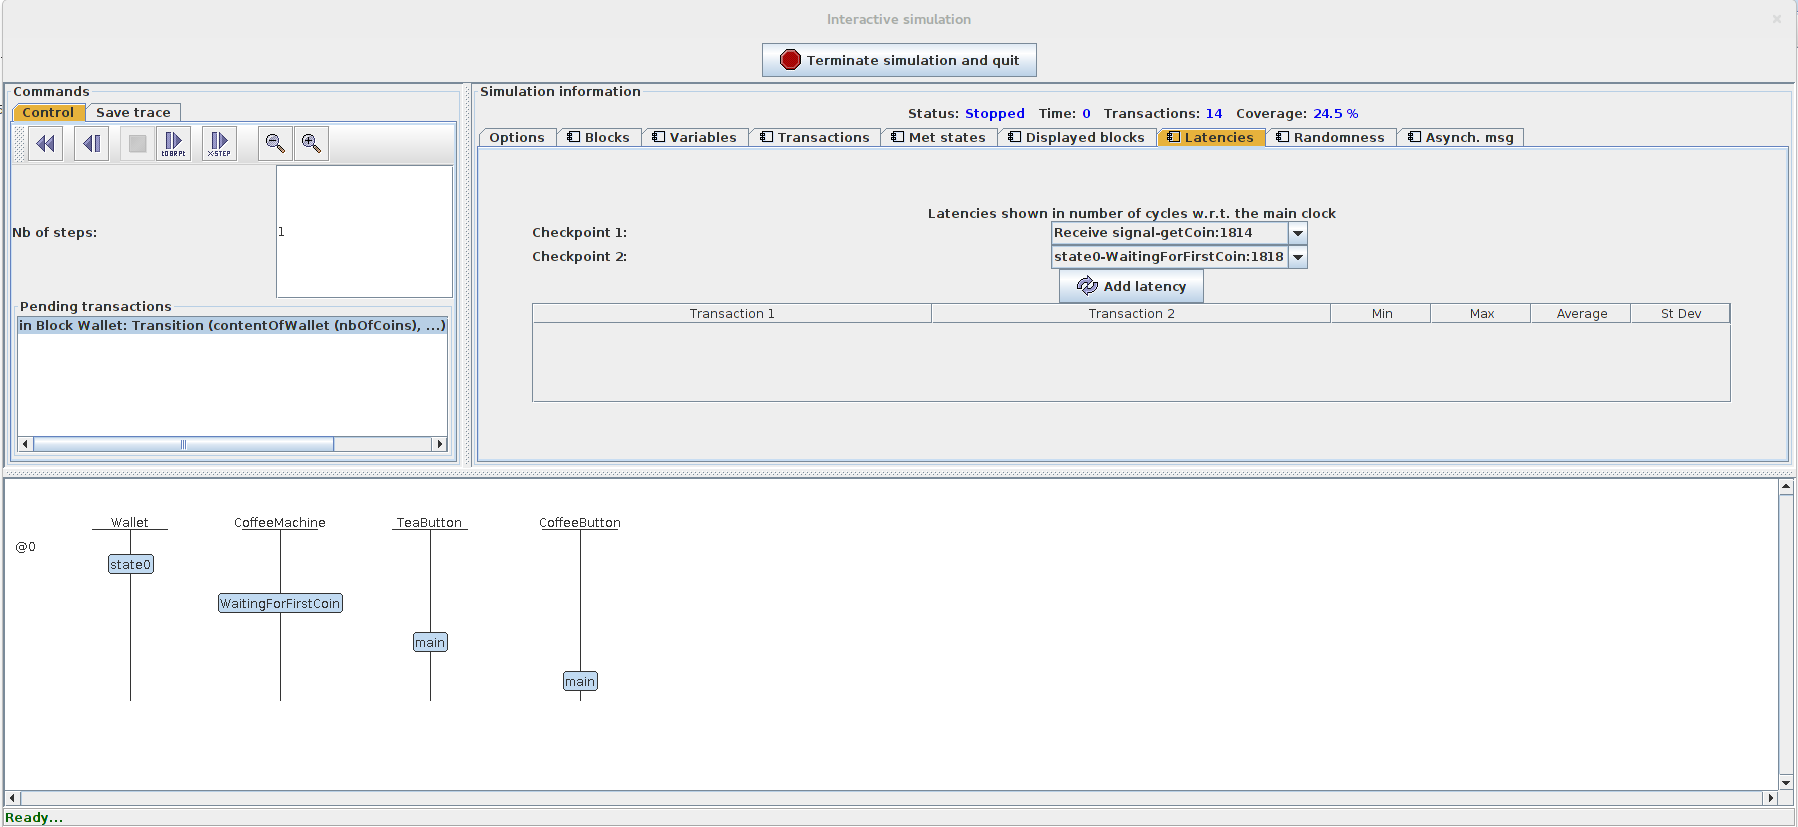
\includegraphics[width=0.99\textwidth]{fig/latencymeasure.png}
\caption{Latency Measurement Panel} \label{fig:latencymeasurement}
\end{figure*}

After syntax analysis, run interactive simulation, and then on the Latency Panel (Figure \ref{fig:latencymeasurement}), we indicate that we should measure the latency between these two checkpoints by selecting the operators and clicking the `Add latency' button. After running 100 steps of the simulation, the minimum, maximum, average, standard deviation of the latency measurements is displayed as shown in Figure \ref{fig:latencyresults}.

\begin{figure*}[htbp]
\centering
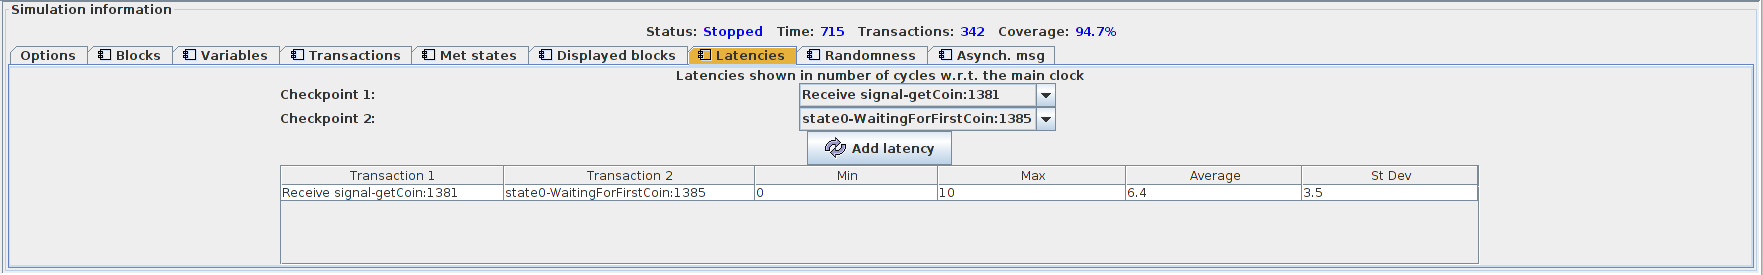
\includegraphics[width=0.99\textwidth]{fig/latencyresults.png}
\caption{Latency Results} \label{fig:latencyresults}
\end{figure*}


\section{Conclusion}

	All in all, TTool is a useful software, which allows the user to generate systems using SysML. By guiding the user through each of the steps of the process (Methodology, Assumptions, Requirements, Analysis and Design) it serves as a platform for better structured, and comprehensive designs. These models provide all the information required to understand the present state of the design and enable easy changes in the future. It is straightforward and intuitive and it has many more features than the ones shown in this manual, therefore making it a very complete tool in the development and simulation of engineering designs. 
	
\end{document}
